\begin{figure*}
  \centering
  %\begin{subfigure}{0.32\textwidth}
  %  \includegraphics[width=\textwidth]{figures/pdfs/XctLatency/TATP.pdf}
  %  \caption{TATP}
  %  \label{fig::XctLatency::TATP}
  %\end{subfigure}
  %\begin{subfigure}{0.32\textwidth}
  %  \includegraphics[width=\textwidth]{figures/pdfs/XctLatency/TPCB.pdf}
  %  \caption{TPCB}
  %  \label{fig::XctLatency::TPCB}
  %\end{subfigure}
  %\begin{subfigure}{0.32\textwidth}
  %  \includegraphics[width=\textwidth]{figures/pdfs/XctLatency/TPCC.pdf}
  %  \caption{TPCC}
  %  \label{fig::XctLatency::TPCC}
  %\end{subfigure}
  \subfigure[TATP -- Update Location]{\label{fig::XctLatency::TATP} 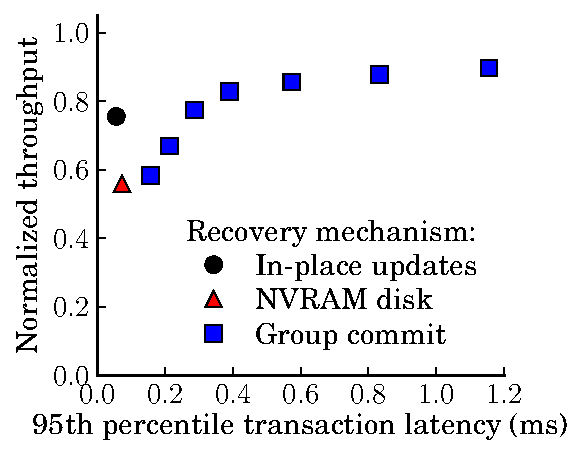
\includegraphics[width=.49\textwidth]{OLTP_eval/XctLatency_TATP.pdf}}
  \subfigure[TPCB]{\label{fig::XctLatency::TPCB}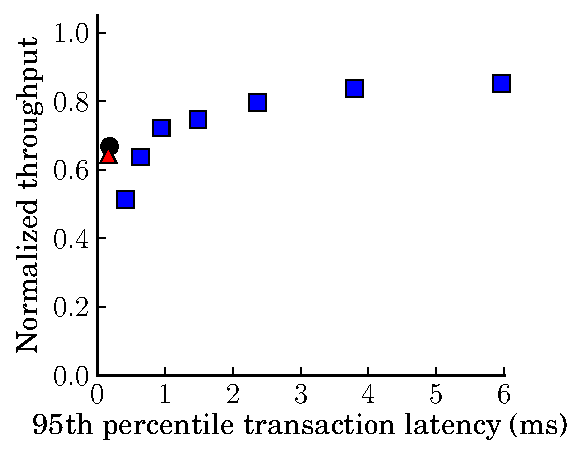
\includegraphics[width=.49\textwidth]{OLTP_eval/XctLatency_TPCB.pdf}}
  \subfigure[TPCC -- New Order]{\label{fig::XctLatency::TPCC}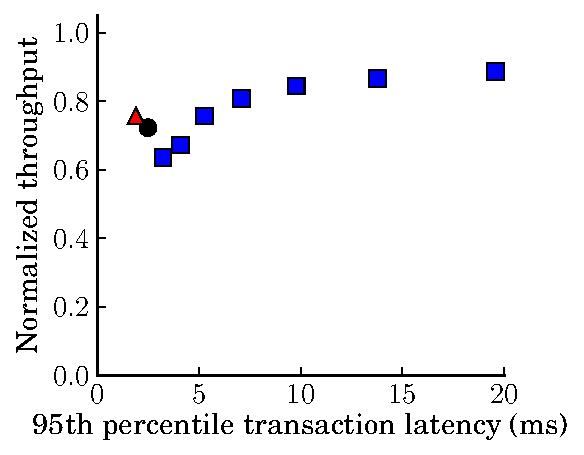
\includegraphics[width=.49\textwidth]{OLTP_eval/XctLatency_TPCC.pdf}}
  \caption{\textbf{95th percentile transaction latency.} All graphs are normalized to 0\textmu s persist barrier latency \InPlace throughput.  Experiments use 3\textmu s persist barrier latency.  \GroupCommit avoids high latency persist barriers by defering transaction commit, committing entire batches atomically.}
  \label{fig::XctLatency}
\end{figure*}
